\documentclass[../main.tex]{subfiles}

\begin{document}
This section will not cover all of the details of SGX, but only those
applicable to our project; for a complete treatment of SGX please
refer to~\cite{IntelCorporation2010}. \Intel~SGX is a set of x86
instructions that allow for a programming model wherein a program can
be split into two components: an untrusted component that executes as
normal and a trusted component that executes within a protected area
of RAM, called an enclave. 

The protection of an enclave is managed by the CPU; any data written
to the enclave is encrypted first by a memory encryption engine
(implemented in hardware) and is only decrypted when required by the
CPU during the execution of the trusted component, which we refer to
as the \textit{enclave program}, to which that enclave belongs. The
key used for this encryption process is derived from a combination of
a device key, unique to each SGX-enabled CPU and the ``identity'' of
the enclave (MRENCLAVE), a cryptographic hash of the enclave's
contents at the \textit{enclave program}'s initialization. SGX thus
ensures that no process, other than the one that initialized the
enclave, may access the protected area.

Interacting with the \textit{enclave program}, as a result, may only occur
through invoking a programmer defined interface, called a callgate, as
depicted in Figure~\ref{fig:sgxhighlevel}.

\begin{figure}[H]
  \centering
  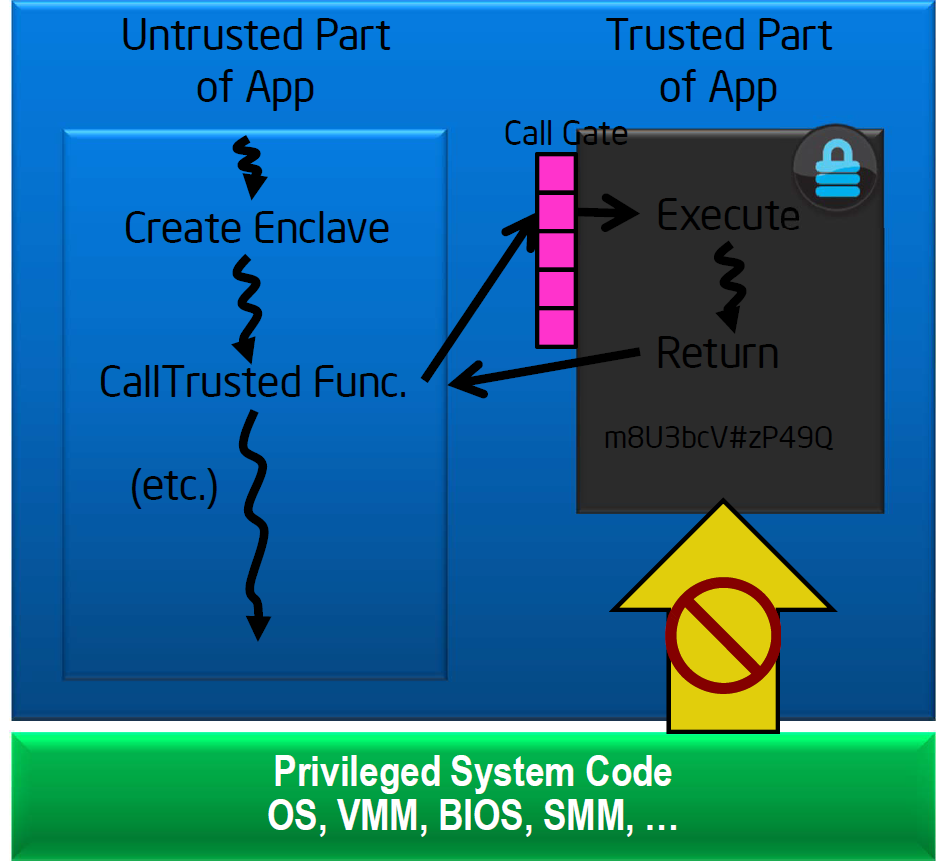
\includegraphics[scale=0.25]{images/sgxhighlevel.png}
  \caption{Interaction of the untrusted part of the application with
    the trusted part can only occur through a callgate}
  \label{fig:sgxhighlevel}
\end{figure}
%%%%%%%%%%%%% transition to OpenSGX still have to add more to the SGX
%%%%%%%%%%%%% overview

\subsubsection{Initialising an SGX Enclave}

Launching an SGX \textit{enclave program} requires the execution of
the following steps:

\begin{enumerate}
  \item The \textit{enclave program} is first compiled and then signed
    with an \Intel~ verified certificate\footnote{While the requirements
    imposed on the certificate for successful verification are well
    documented, the process is not automated, and involves an application
    to \Intel's Infrastruction Attestation Service (IAS)}. The signing
    process generates a data structure called \texttt{SIGSTRUCT} that
    contains the aforementioned MRENCLAVE, the identity of the signing
    entity, MRSIGNER, and the signature across this structure.
  \item When attempting to launch the \textit{enclave program}, the
    CPU calculates MRENCLAVE using priveleged SGX instructions, calculates
    MRSIGNER by taking the hash of the public key contained in the signing
    entity's certificate, and then attempts to verify that
    MRSIGNER$_{calc}$ is equal to MRSIGNER$_{SIGSTRUCT}$,
    MRENCLAVE$_{calc}$ is equal to MRENCLAVE$_{SIGSTRUCT}$, and that the
    signature across \texttt{SIGSTRUCT} was generated by the signing
    entity indicated by MRSIGNER.
  \item If all previous checks complete successfully, then the CPU
    proceeds to execute the \textit{enclave program} otherwise, the CPU
    aborts execution.
\end{enumerate}

At the time we begun working on this project we did not posses access
to SGX hardware, forcing us to use a simulator. There were two
choices, at the time: OpenSGX and the \Intel~ Windows SDK's simulation
mode. We selected the former to implement our prototype as it was
compatible with Linux, a platform we were more familiar with, and had
several examples we could refer to for guidance in our implementation
(the Intel SDK, at the time, was under-documented). The following
section provides a quick examination of OpenSGX's salient features.


\subsubsection{Brief Notes on OpenSGX}
\subfile{sections/opensgx.tex}
\end{document}

%%% Local Variables:
%%% mode: latex
%%% TeX-master: "../main"
%%% End:
